%%%%%%%%%%%%%%%%%%%%%%%%%%%%%%% beamer %%%%%%%%%%%%%%%%%%%%%%%%%%%%%%%%%%%%%%%%%%%%%%%%%
% To run - pdflatex filename.tex
%      acroread filename.pdf
%%%%%%%%%%%%%%%%%%%%%%%%%%%%%%%%%%%%%%%%%%%%%%%%%%%%%%%%%%%%%%%%%%%%%%%%%%%%%%%%%%%%%%%%

\documentclass[compress,oilve]{beamer}
\mode<presentation>

\usetheme[]{CambridgeUS}
% other themes: AnnArbor, Antibes, Bergen, Berkeley, Berlin, Boadilla, boxes, CambridgeUS, Copenhagen, Darmstadt, default, Dresden, Frankfurt, Goettingen,
% Hannover, Ilmenau, JuanLesPins, Luebeck, Madrid, Maloe, Marburg, Montpellier, PaloAlto, Pittsburg, Rochester, Singapore, Szeged, classic

\usecolortheme{beaver}
% color themes: albatross, beaver, beetle, crane, default, dolphin,  fly, lily, orchid, rose, seagull, seahorse, sidebartab, whale, wolverine

\usefonttheme{professionalfonts}
% font themes: default, professionalfonts, serif, structurebold, structureitalicserif, structuresmallcapsserif


\hypersetup{pdfpagemode=FullScreen} % makes your presentation go automatically to full screen

% define your own colors:
\definecolor{Red}{rgb}{1,0,0}
\definecolor{Blue}{rgb}{0,0,1}
\definecolor{Green}{rgb}{0,1,0}
\definecolor{magenta}{rgb}{1,0,.6}
\definecolor{lightblue}{rgb}{0,.5,1}
\definecolor{lightpurple}{rgb}{0.8, 0.6, 0.9}
\definecolor{gold}{rgb}{.6,.5,0}
\definecolor{orange}{rgb}{1,0.4,0}
\definecolor{hotpink}{rgb}{1,0,0.5}
\definecolor{newcolor2}{rgb}{.5,.3,.5}
\definecolor{newcolor}{rgb}{0,.3,1}
\definecolor{newcolor3}{rgb}{1,0,.35}
\definecolor{darkgreen1}{rgb}{0, .35, 0}
\definecolor{darkgreen}{rgb}{0, .6, 0}
\definecolor{darkred}{rgb}{.75,0,0}
\definecolor{skyblue}{HTML}{75bbfd}

\definecolor{olive}{cmyk}{0.64,0,0.95,0.4}
\definecolor{purpleish}{cmyk}{0.75,0.75,0,0}

% can also choose different themes for the "inside" and "outside"

% \usepackage{beamerinnertheme_______}
% inner themes include circles, default, inmargin, rectangles, rounded

% \usepackage{beamerouterthemesmoothbars}
% outer themes include default, infolines, miniframes, shadow, sidebar, smoothbars, smoothtree, split, tree


\useoutertheme[subsection=true, height=40pt]{smoothbars}

% to have the same footer on all slides
%\setbeamertemplate{footline}[text line]{STUFF HERE!}
\setbeamertemplate{footline}[text line]{} % makes the footer EMPTY
% include packages
%

%show the page numbers in footnote
%\addtobeamertemplate{navigation symbols}{}{%
%	\usebeamerfont{footline}%
%	\usebeamercolor[fg]{footline}%
%	\hspace{1em}%
%	\insertframenumber/\inserttotalframenumber
%}

\setbeamercolor{footline}{fg=purpleish}
\setbeamerfont{footline}{series=\bfseries}

%add color to curent subsection
\setbeamertemplate{section in head/foot}{\hfill\tikz\node[rectangle, fill=darkred, rounded corners=1pt,inner sep=1pt,] {\textcolor{white}{\insertsectionhead}};}
\setbeamertemplate{section in head/foot shaded}{\textcolor{darkred}{\hfill\insertsectionhead}}

% Remove bullet of subsections
\setbeamertemplate{headline}
{%
	\begin{beamercolorbox}{section in head/foot}
		\insertsectionnavigationhorizontal{\textwidth}{}{}
	\end{beamercolorbox}%
}


% modify headlline, specially headline size
\setbeamertemplate{headline}{%
	\leavevmode%
	\hbox{%
		\begin{beamercolorbox}[wd=\paperwidth,ht=3.5ex,dp=1.125ex]{palette quaternary}%
			\insertsectionnavigationhorizontal{\paperwidth}{}{\hskip0pt plus1filll}
		\end{beamercolorbox}%
	}
}

\setbeamertemplate{footline}{%
	\leavevmode%
	\hbox{\begin{beamercolorbox}[wd=.5\paperwidth,ht=2.5ex,dp=1.125ex,leftskip=.3cm plus1fill,rightskip=.3cm]{author in head/foot}%
			\usebeamerfont{author in head/foot}\insertshortauthor ~ \insertshortinstitute
		\end{beamercolorbox}%
		\begin{beamercolorbox}[wd=.5\paperwidth,ht=2.5ex,dp=1.125ex,leftskip=.3cm,rightskip=.3cm plus1fil]{title in head/foot}%
			\usebeamerfont{title in head/foot}\insertshorttitle\hfill\insertframenumber\,/\,\inserttotalframenumber
	\end{beamercolorbox}}%
	\vskip0pt%
}


%\setbeamertemplate{navigation symbols}{}

\title{Word Embedding}
\author{ML Instruction Team, Fall 2022}
\institute[]{CE Department \newline  Sharif University of Technology \newline \newline}
\date[\today]{}
%\titlegraphic{\includegraphics[scale=.35]{example-image}}



%Write \usepackage{etex} just after the \documentclass line (it should be the first loaded package).
\usepackage{etex}
\usepackage{subcaption}
\usepackage{multicol}
\usepackage{amsmath}
\usepackage{epsfig}
\usepackage{graphicx}
\usepackage{mathtools}
\usepackage[all,knot]{xy}
\xyoption{arc}
\usepackage{url}
\usepackage{multimedia}
\usepackage{hyperref}
\hypersetup{colorlinks,linkcolor=blue,citecolor=redorange,urlcolor=darkred}
\usepackage{multirow}
\usepackage[font={scriptsize}]{caption}
\usepackage{pgf}
\usepackage{fontspec}
%\setsansfont[Scale=MatchLowercase, BoldFont = * Bold, ItalicFont = * Italic]{Caladea}

%\usepackage{enumitem,xcolor}
%\newcommand{\labelitemi}{$\blacksquare$}
%\newcommand{\labelitemii}{$\diamond$}
%\newcommand{\labelitemiii}{$\square$}
%\newcommand{\labelitemiv}{$\ast$}
%\setbeamercolor*{item}{fg=red}


\usefonttheme{professionalfonts} 
\setbeamertemplate{itemize item}{\color{skyblue}$\blacksquare$}
\setbeamertemplate{itemize subitem}{\color{hotpink}$\blacktriangleright$}
\setbeamertemplate{itemize subsubitem}{\color{orange}$\bullet$}


\usepackage{anyfontsize}
\usepackage{t1enc}
\usepackage{tikz}
\usetikzlibrary{calc,trees,positioning,arrows,chains,shapes.geometric,decorations.pathreplacing,decorations.pathmorphing,shapes,matrix,shapes.symbols}



\newtheorem{proposition}[theorem]{Proposition}
\newtheorem{remark}[theorem]{Remark}
\newtheorem{assumption}[theorem]{Assumption}

\usepackage{xcolor}
\newcommand{\tc}[2]{
	\textcolor{#1}{#2}
}

%\usepackage{fontspec, unicode-math}
%\setmainfont[Scale=0.9]{Nimbus Roman No9 L}
%\setmonofont[Scale=0.9]{Monaco}
\setsansfont[Scale=1]{Times New Roman}

\newcommand{\vect}[1]{\boldsymbol{#1}}

\definecolor{strings}{rgb}{.624,.251,.259}
\definecolor{keywords}{rgb}{.224,.451,.686}
\definecolor{comment}{rgb}{.322,.451,.322}


%\usepackage{smartdiagram}
%\usesmartdiagramlibrary{additions}
%%%%%%%%%%%%%%%%%%%%%%%%%%%%%%%%%%%%%%%%%%%%%%%%%%%%%%%%%%%%%%%%%%%%%%%%%%%%%%%%%%%%%%%%%%%%
%%%%%%%%%%%%%%%%%%%%%%%%%%%%%% Title Page Info %%%%%%%%%%%%%%%%%%%%%%%%%%%%%%%%%%%%%%%%%%%
%%%%%%%%%%%%%%%%%%%%%%%%%%%%%%%%%%%%%%%%%%%%%%%%%%%%%%%%%%%%%%%%%%%%%%%%%%%%%%%%%%%%%%%%%%


%%%%%%%%%%%%%%%%%%%%%%%%%%%%%%%%%%%%%%%%%%%%%%%%%%%%%%%%%%%%%%%%%%%%%%%%%%%%%%%%%%%%%%%%%%
%%%%%%%%%%%%%%%%%%%%%%%%%%%%%% Begin Your Document %%%%%%%%%%%%%%%%%%%%%%%%%%%%%%%%%%%%%%%
%%%%%%%%%%%%%%%%%%%%%%%%%%%%%%%%%%%%%%%%%%%%%%%%%%%%%%%%%%%%%%%%%%%%%%%%%%%%%%%%%%%%%%%%%%
%%%%%%%%%%%%%%%%%%%%%%%%%%%%%%%%%%%%%%%%%%%%%%%%%%%%%%%%%%%%%%%%%%%%%%%%%%%%%%%%%%%%%%%%%%
%%%%%%%%%%%%%%%%%%%%%%%%%%%%%% Begin Your Document %%%%%%%%%%%%%%%%%%%%%%%%%%%%%%%%%%%%%%%
%%%%%%%%%%%%%%%%%%%%%%%%%%%%%%%%%%%%%%%%%%%%%%%%%%%%%%%%%%%%%%%%%%%%%%%%%%%%%%%%%%%%%%%%%%
\begin{document}
	
%%%%%%%%%%%%%%%%%%%%%%%%%%%%%%%%%%%%%%%%%%%%%%%%%%%%%%%%%%%%%%%%%%%%%%%%%%%%%%%%%%%%%%%%%%
	\fontsize{9}{9}
\begin{frame}[noframenumbering, plain]
	\titlepage
\end{frame}

%%%%%%%%%%%%%%%%%%%%%%%%%%%%%%%%%%%%%%%%%%%%%%%%%%%%%%%%%%%%%%%%%%%%%%%%%%%%%%%%%%%%%%%%%%
\section{Introduction}
%%%%%%%%%%%%%%%%%%%%%%%%%%%%%%%%%%%%%%%%%%%%%%%%%%%%%%%%%%%%%%%%%%%%%%%%
\frame{\frametitle{How to Represent Texts?}

\begin{itemize}
	\item Consider the below sentences

	\begin{itemize}
		\item Today is a beautiful day.
		\item Tomorrow will be a better day.
	\end{itemize}

	\item How can we represent the word tomorrow and what should the representation indicate?
	\item Some classic methods
 	\begin{itemize}
		\item Assigning an id to each word
		\item One-Hot encoding
		\item Co-Occurrence matrix
	\end{itemize}

    \begin{figure}[!h]
    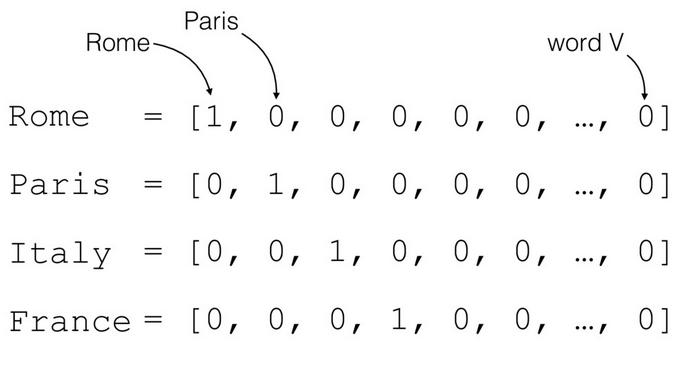
\includegraphics[width=5cm]{Figs/one-hot.png}
    \caption{One-Hot Encoding, \href{https://medium.com/intelligentmachines/word-embedding-and-one-hot-encoding-ad17b4bbe111} 
            {Source}}
    \end{figure}
        
\end{itemize}	

}

\section{Co-Occurrence Matrix}
\frame{\frametitle{Co-Occurrence Matrix}

\begin{itemize}
	\item Example

	\begin{itemize}
		\item I like deep learning.  
		\item I like NLP.
		\item I enjoy flying.
	\end{itemize}

    \begin{figure}[!h]
    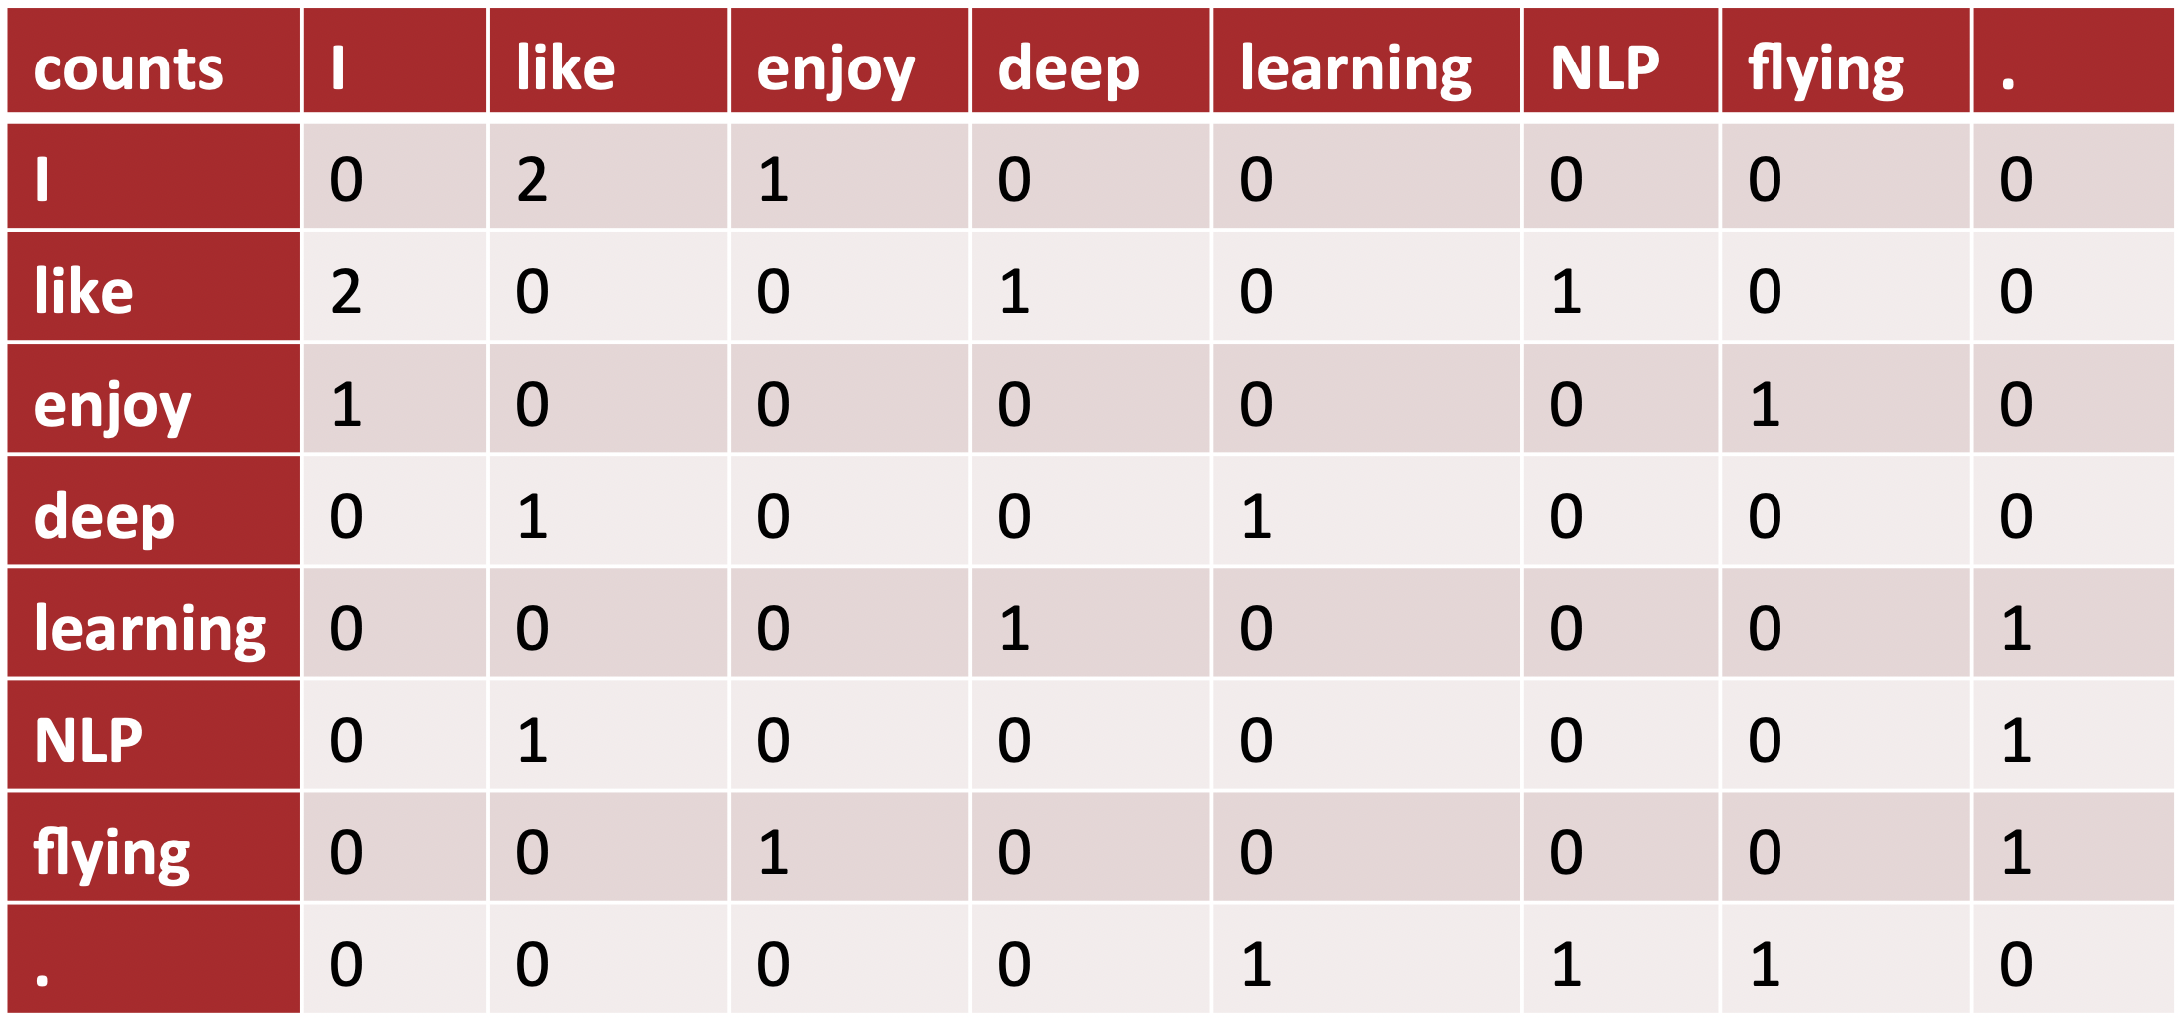
\includegraphics[width=9cm]{Figs/co-occur.png}
    \caption{Co-Occurrence Matrix, \href{https://cs224d.stanford.edu/lectures/CS224d-Lecture2.pdf} 
            {Source}}
    \end{figure}
        
\end{itemize}	

}

\section{Bag of Words}
\frame{\frametitle{Bag of Words (BoW)}

\begin{itemize}
	\item It is an approach used widely in information retrieval.
	\item BoW is based on counting occurrence of words in each text. 
	\item Each word is represented by the documents it occurs in. 
	\item It is called Bag of Words because it does not consider the \tc{keywords}{order} of words.
	\item But does it convey a meaning?

	\begin{figure}[!h]
    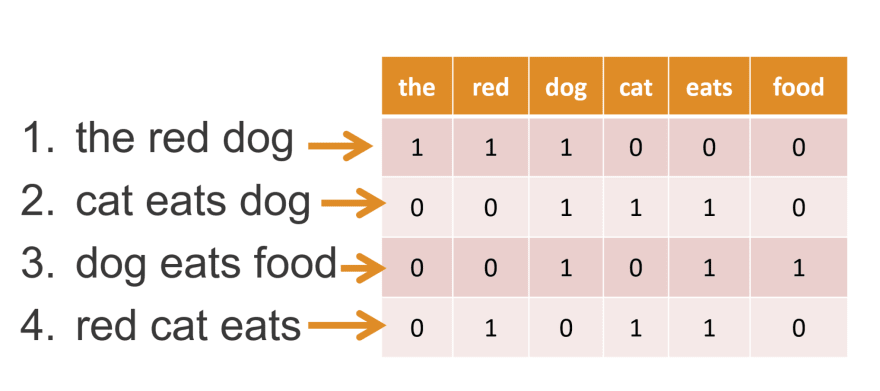
\includegraphics[width=8cm]{Figs/bow.png}
    \caption{Example of BoW method, \href{https://medium.com/swlh/spam-filtering-using-bag-of-words-aac778e1ee0b} 
            {Source}}
    
    \end{figure}
        
\end{itemize}	

}

\section{Continuous Bag of Words}
\frame{\frametitle{Continuous Bag of Words (CBoW)}
\begin{itemize}
    \item To obtain a meaning for each word, a \tc{keywords}{fake task} should be defined. 
    \item Consider the following incomplete sentence
    \begin{center}
        S $\coloneqq$ I prefer to travel by ... rather than cars.
    \end{center}
    \item By using which one of the words flowers, airplanes, or lions should we fill in the above sentence? The most probable one!
    \begin{equation*}
        \underset{w \in \text{\{flowers, airplanes, lions\}}}{\mathbin{argmax}}
        P(w_i=w|S)
    \end{equation*}
    \item What if a sentence is too long? How should we deal with alternative length of sentences? Use a \tc{keywords}{window}. (It comes from an assumption that to guess a word, its neighbourhood should be enough.)
    \begin{equation*}
        \underset{w \in \text{\{flower, airplane, lion\}}}{\mathbin{argmax}}
        P(w_i=w|w_{i - l}, w_{i - l + 1}, ..., w_{i-1}, w_{i+1}, ..., w_{i + l - 1}, w_{i + l})
    \end{equation*}
    \item How to calculate the probabilities given a \tc{keywords}{corpus}?
    
\end{itemize}
	
% 	\begin{figure}[!h]
%     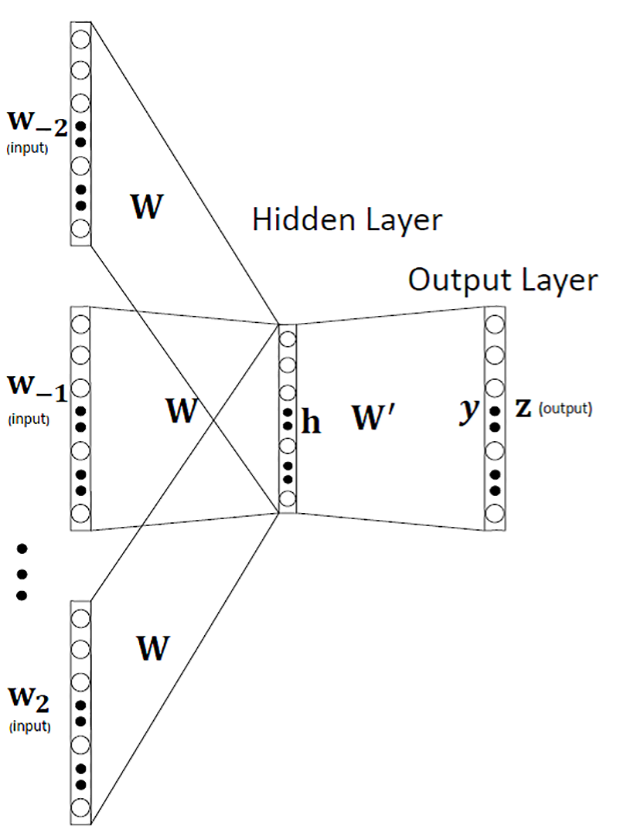
\includegraphics[width=5cm]{Figs/cbow.png}
%     \caption{Example of CBoW method, \href{https://medium.com/swlh/spam-filtering-using-bag-of-words-aac778e1ee0b} 
%             {Source}}
    
%     \end{figure}

}
\frame{\frametitle{Continuous Bag of Words (CBoW)}
	
	\begin{figure}[!h]
    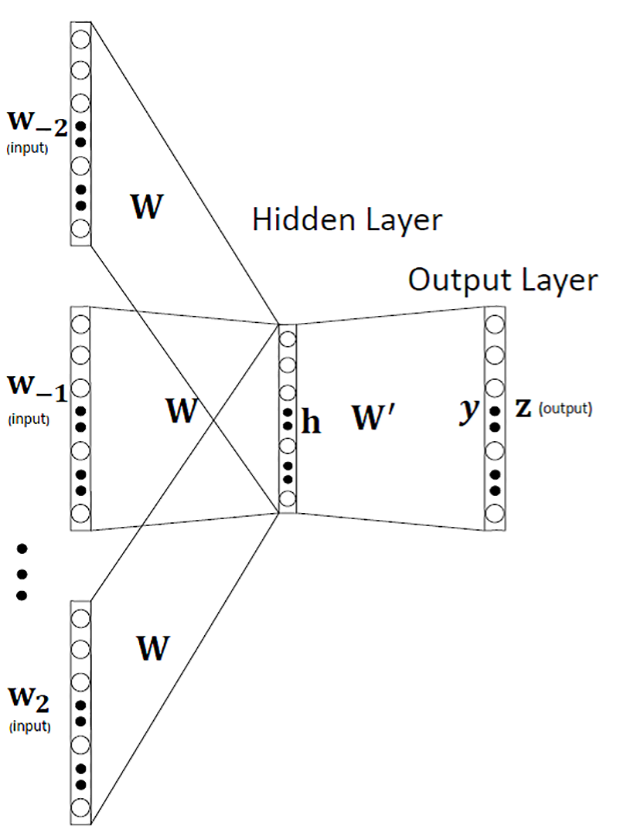
\includegraphics[width=4.5cm]{Figs/cbow.png}
    \caption{CBoW model, \href{https://doi.org/10.1371/journal.pone.0216636.g001} 
            {Source}}
    
    \end{figure}
    \begin{itemize}
        \item Note that matrix W is \tc{keywords}{shared}. (The order is not important)
    \end{itemize}

}

\frame{\frametitle{Continuous Bag of Words (CBoW)}
    \begin{itemize}
        \item Considering the fake task defined earlier, how can we represent a word in a meaningful way? Hidden layer matrix. (\tc{keywords}{Matrix W})
        \item By determining the number of the hidden layer neurons (as hyper parameter m), each word is represented by a \tc{keywords}{m-dimension} vector.
        
    \end{itemize}
	
	\begin{figure}[!h]
    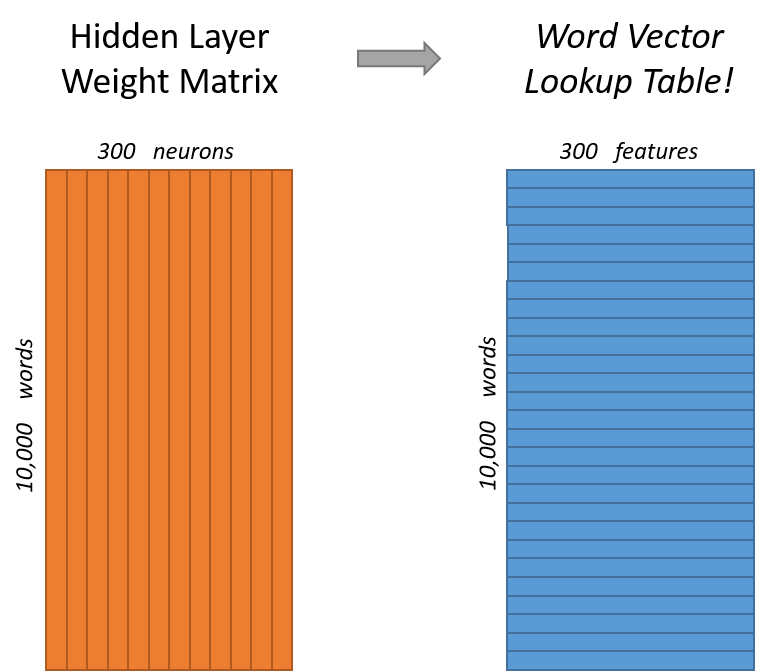
\includegraphics[width=5cm]{Figs/W_matrix.png}
    \caption{Obtained Feature Vector, \href{https://towardsdatascience.com/word2vec-skip-gram-model-part-1-intuition-78614e4d6e0b} 
            {Source}}
    
    \end{figure}

}

\section{Skip-gram}
\frame{\frametitle{Skip-gram}

\begin{itemize}
	\item It is similar to CBoW and just the fake task is inverted. (Here \tc{keywords}{matrix W} is the word embedding matrix)
\end{itemize}
\begin{figure}[!h]
    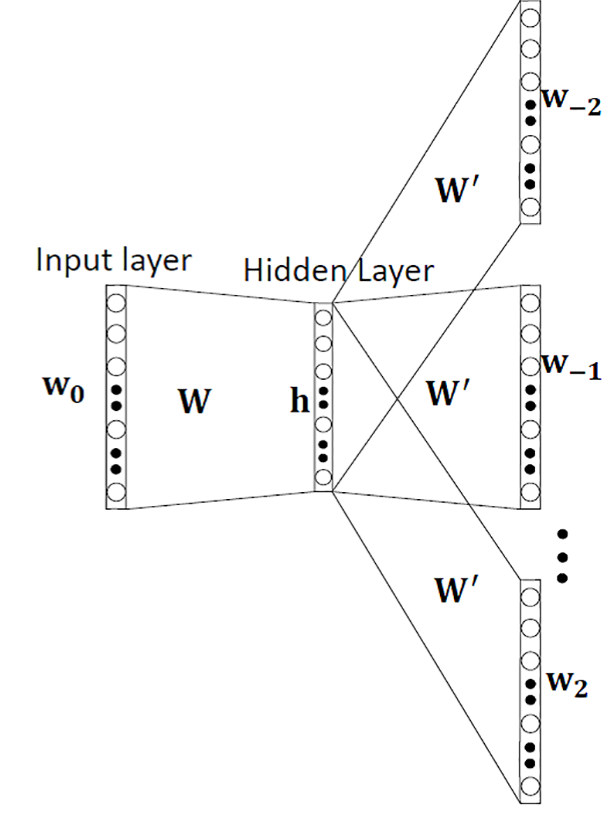
\includegraphics[width=4cm]{Figs/skip-gram.png}
    \caption{Skip-gram model, \href{https://doi.org/10.1371/journal.pone.0216636.g001} 
            {Source}}
    
    \end{figure}



}

\frame{\frametitle{Skip-gram}
\begin{itemize}
    \item \textbf{Example} (Source text: The man who \tc{keywords}{passes} the sentence should swing the sword.)
\end{itemize}
    
    \begin{figure}[!h]
    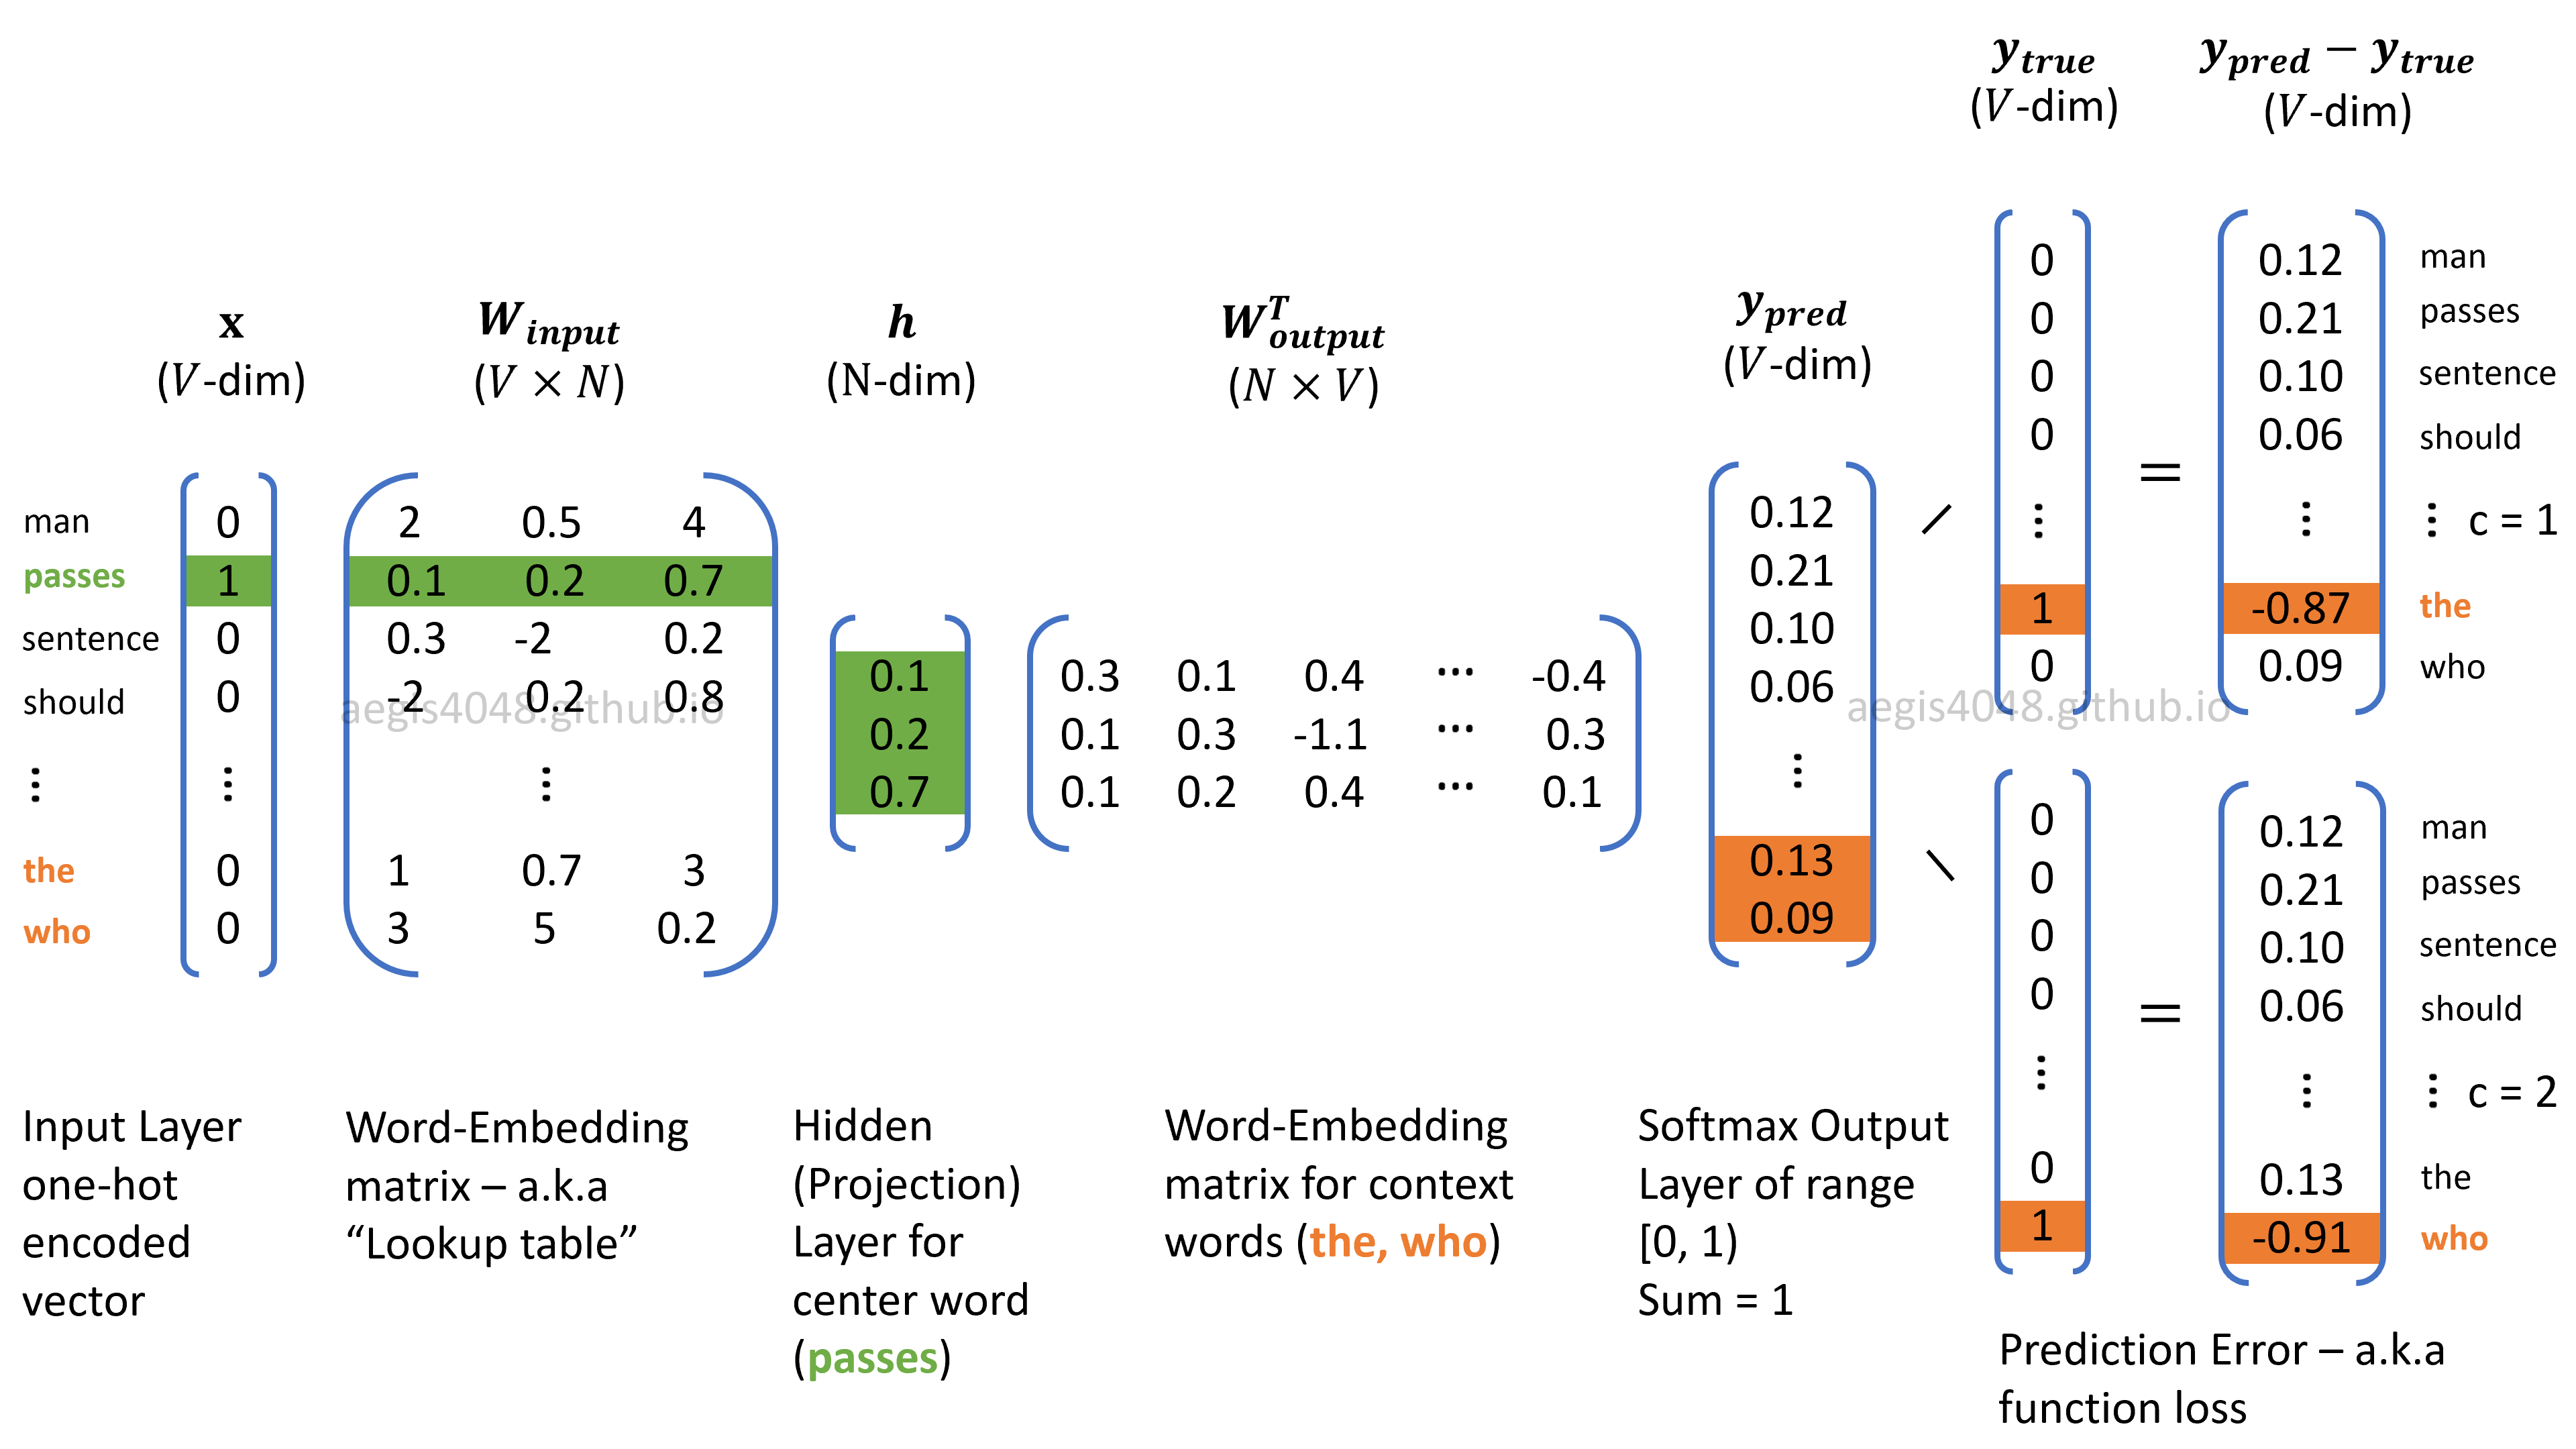
\includegraphics[width=10cm]{Figs/example2.png}
    \caption{Skip-gram Method for Window Size 1 Centered Word passes, \href{https://aegis4048.github.io/demystifying_neural_network_in_skip_gram_language_modeling} 
            {Source}}
    
    \end{figure}
        
}





% \section{One Hot Embedding}
% %%%%%%%%%%%%%%%%%%%%%%%%%%%%%%%%%%%%%%%%%%%%%%%%%%%%%%%%%%%%%%%%%%%%%%%%
% \frame{\frametitle{Backpropagation Through Time (BPTT)}
	
% \begin{figure}[!h]
% 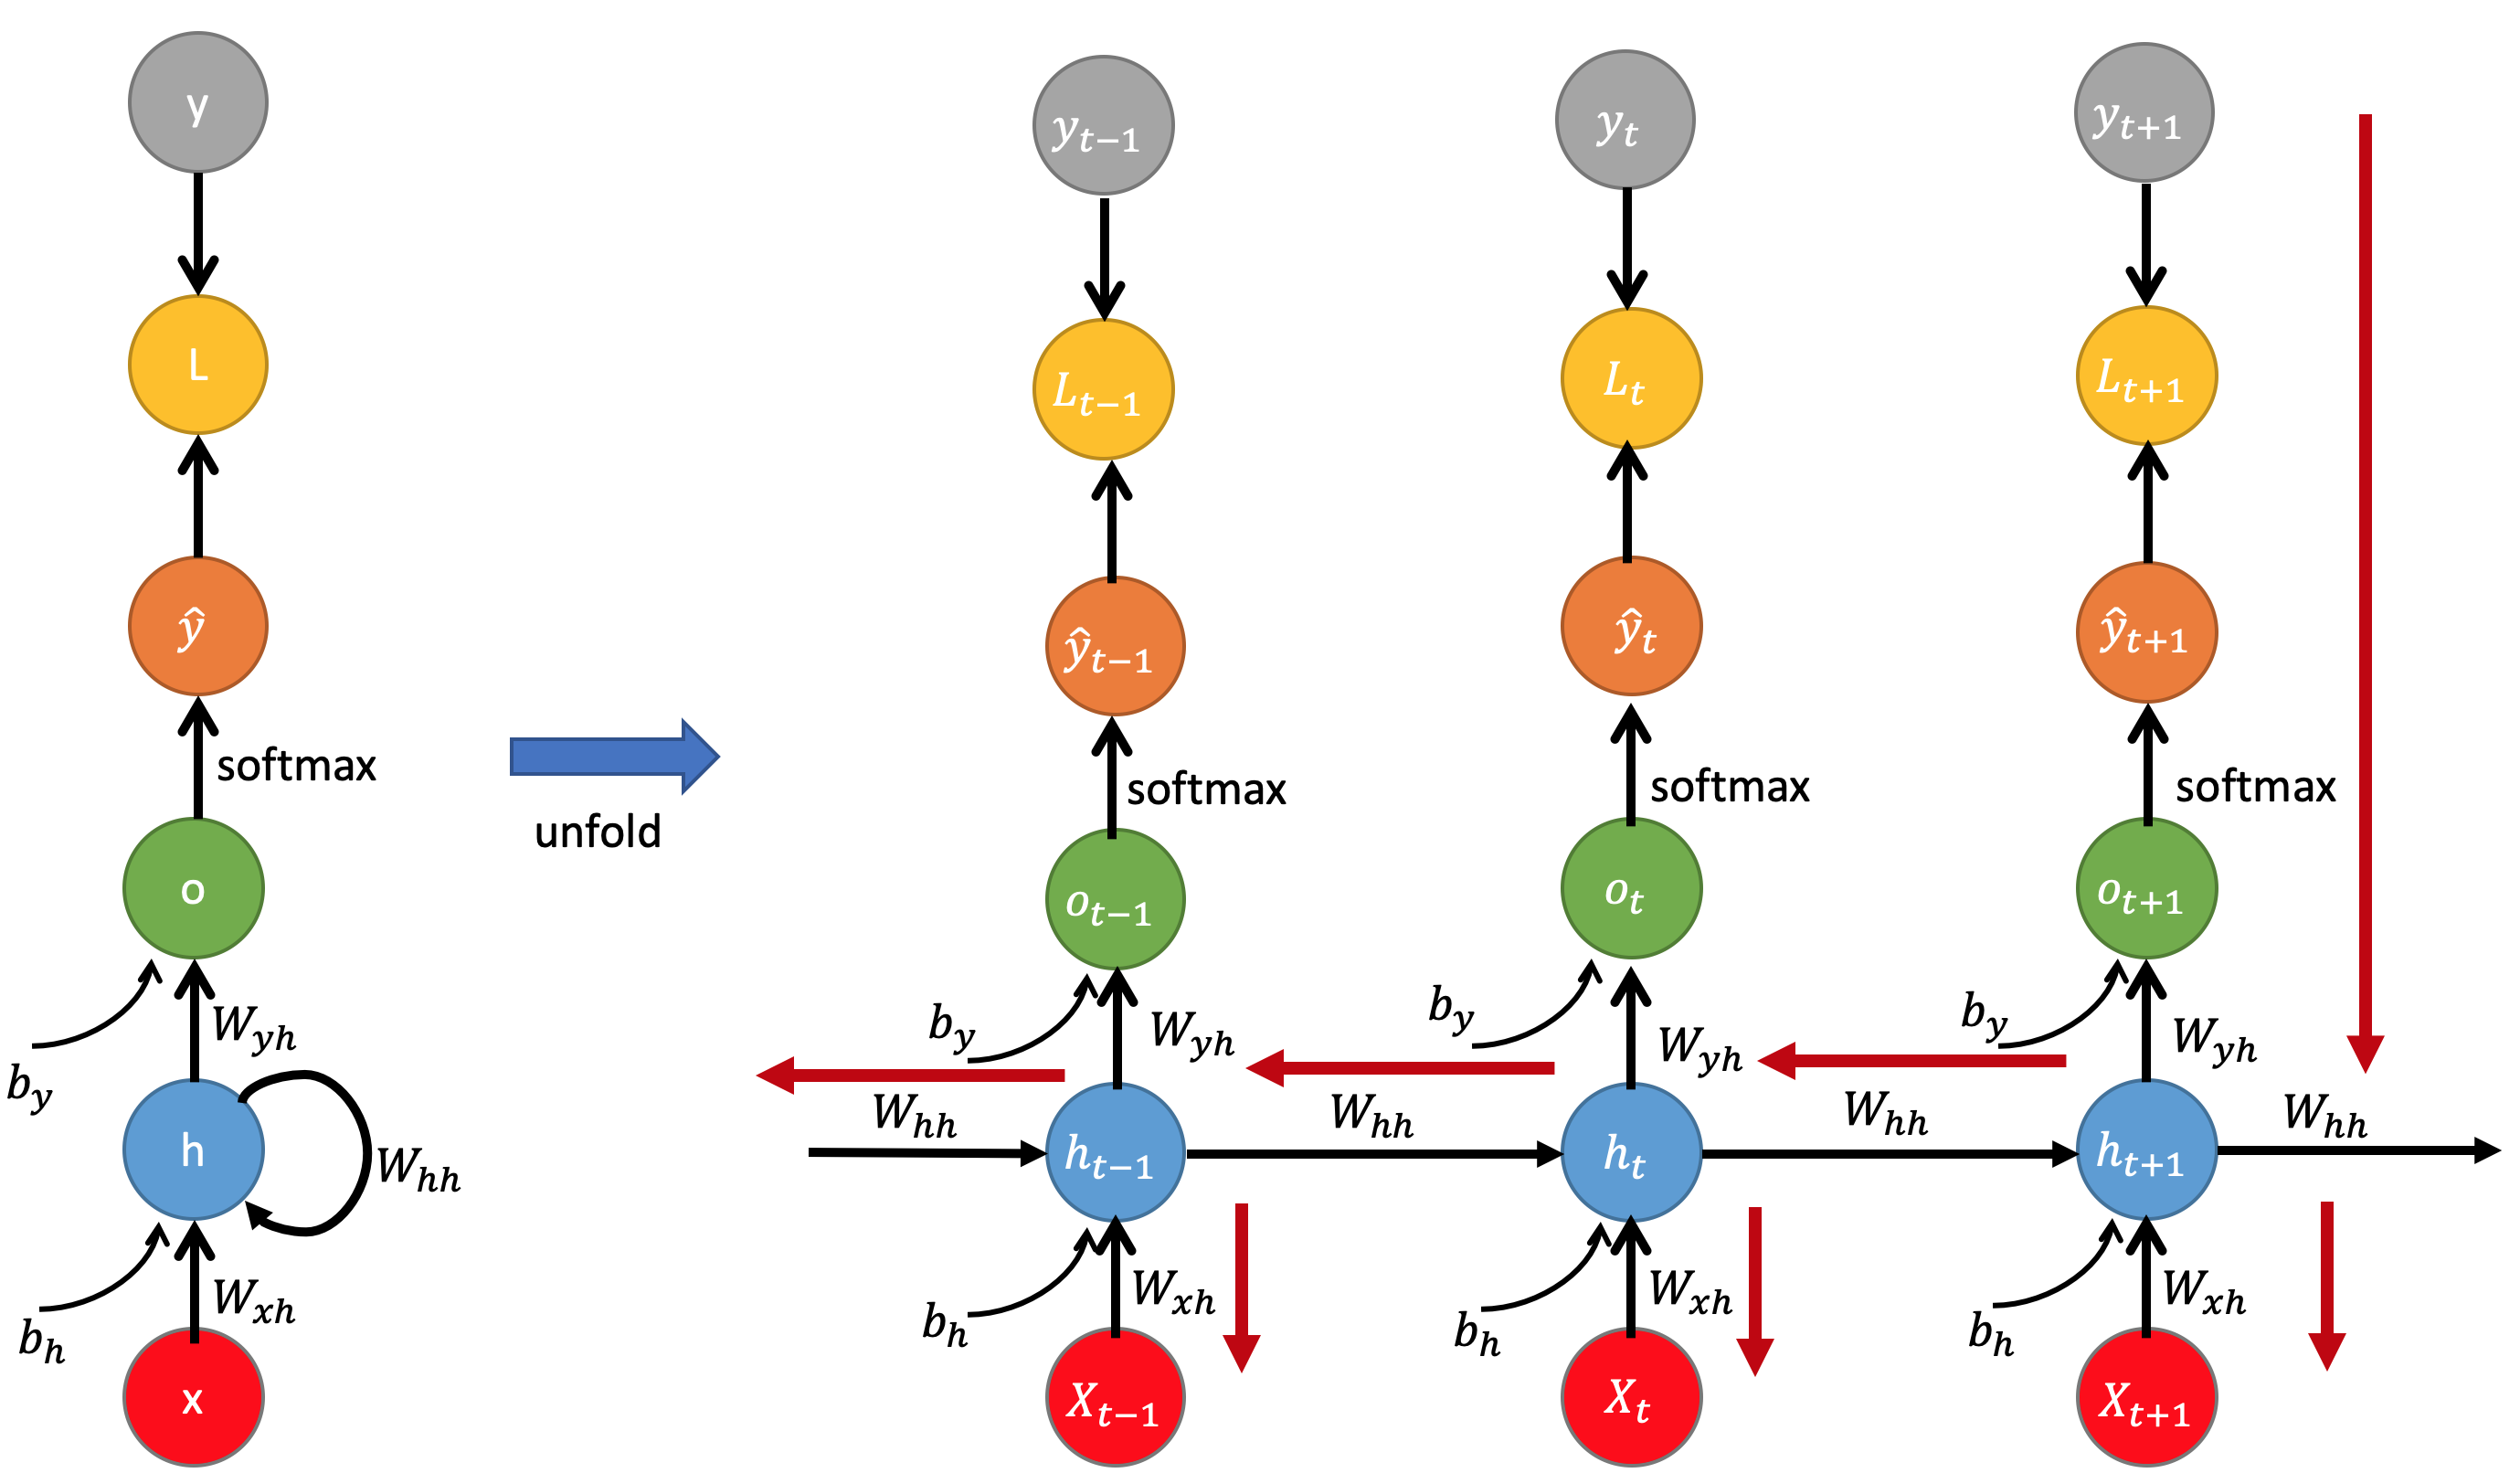
\includegraphics[width=10cm]{Figs/BPTT.png}
% \caption{Simple RNN Computational Graph, \href{https://mmuratarat.github.io/2019-02-07/bptt-of-rnn} 
%         {Source}}

% \end{figure}

% }


\frame{\frametitle{References}
\vspace{-1cm}
% \begin{itemize}
\bibliographystyle{plain}
\renewcommand\refname{}
\nocite{*}
\bibliography{cites}
% \item https://lilianweng.github.io/posts/2018-06-24-attention/
% \vspace{3mm}
% \item https://mmuratarat.github.io/2019-02-07/bptt-of-rnn
% \vspace{3mm}
% \item https://d2l.ai/chapter\_recurrent-modern/encoder-decoder.html
% \vspace{3mm}
% \item https://d2l.ai/chapter\_recurrent-modern/seq2seq.html
% \vspace{3mm}
% \item https://d2l.ai/chapter\_recurrent-modern/beam-search.html
% \vspace{3mm}
% \end{itemize}

}
%%%%%%%%%%%%%%%%%%%%%%%%%%%%%%%%%%%%%%%%%%%%%%%%%%%%%%%%%%%%%%%%%%%%%%%%%%%%%%%%%%%%%

\frametitle{Final Notes}
\centering
\vspace{50 pt}
\textbf{Thank You!}
\vspace{50pt}

\textbf{Any Question?}
%%%%%%%%%%%%%%%%%%%%%%%%%%%%%%%%%%%%%%%%%%
\end{document}